\documentclass{beamer}
\graphicspath{ {../images/} }
\usepackage[export]{adjustbox}
\usepackage{tcolorbox}
\newtcbox{\codestyle}{on line,boxrule=0pt,boxsep=0pt,colback=lightgray,top=1pt,bottom=1pt,left=1pt,right=1pt,arc=0pt,fontupper=\ttfamily}

\title{Text to SQL Generation}
\author{Jake Waffle}
\date{2023}

\begin{document}

\frame{\titlepage}

\begin{frame}
\frametitle{Swagger UI}

\adjincludegraphics[trim={{.12\width} {0.3\height} {.5\width} {0.07\height}},clip,scale=0.4]{swagger-ui-example3.png}

\end{frame}

\begin{frame}
\frametitle{Swagger UI}

\adjincludegraphics[trim={{.18\width} {0.11\height} {.1\width} {0.24\height}},clip,scale=0.32]{swagger-ui-example4.png}

\end{frame}


\begin{frame}
\frametitle{Architecture}

\begin{center}
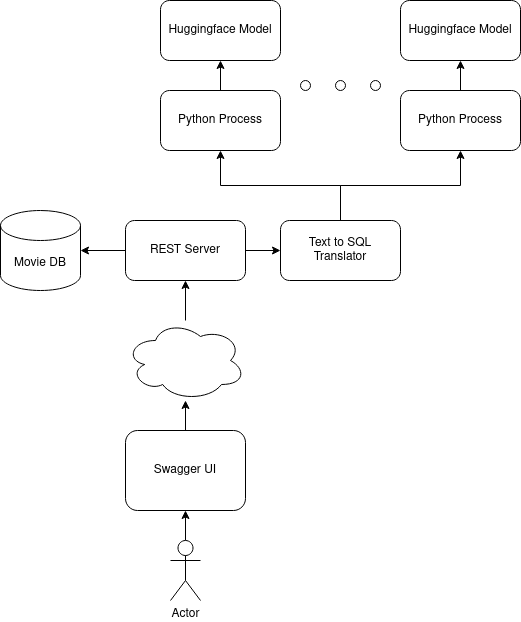
\includegraphics[scale=0.38]{demo-architecture.drawio.png}
\end{center}

\end{frame}

\begin{frame}
\frametitle{Transformer}

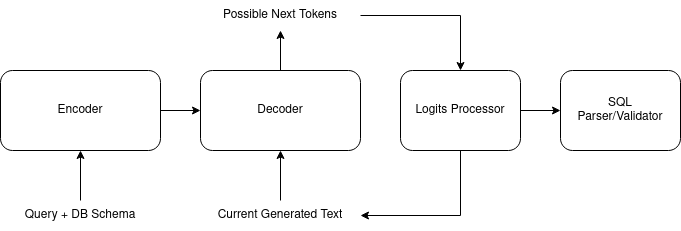
\includegraphics[scale=0.45]{t5-transformer.drawio.png}

\end{frame}

\begin{frame}
\frametitle{Why}

\begin{itemize}[<+->]
  \item Manually supporting filters is maintenance heavy on the frontend/backend
  \item Users don't like learning query languages like OData and reading documentation
  \item The model used isn't trained against a specific database schema
\end{itemize}

\end{frame}

\begin{frame}
\frametitle{Pitfalls}

\begin{itemize}[<+->]
  \item Conventional parsers don't work well with partial word tokens
  \item Text generation support in libraries is generally immature
  \item Python's Global Interpreter Lock interferes with using models in multiple threads (batching and multiple models can alleviate this)
\end{itemize}

\end{frame}

\begin{frame}
\frametitle{Evaluation}

\begin{itemize}[<+->]
  \item Spider text to SQL dataset
  \item Content overlap
\end{itemize}

\end{frame}


\end{document}
